\documentclass[12pt,a4paper]{book}
\usepackage{lmodern}
\usepackage[svgnames]{xcolor} % Required to specify font color
\usepackage{xcolor}
\definecolor{vert1}{rgb}{0.0,0.3.9,0.0}
\definecolor{bleu}{rgb}{0,0,0.5}
\definecolor{bleu3}{rgb}{1,0.2,0.2}
\definecolor{grisgris}{gray}{0.4}
\definecolor{grisclair}{gray}{0.9}
\definecolor{grisfonce}{gray}{0.8}
\definecolor{rougeUPS}{rgb}{0.6, 0.3, 0.3}

\fboxsep =0pt \parindent =0pt\parskip =12pt

\definecolor{ocre}{RGB}{225,0,0}
\definecolor{titlepagecolor}{RGB}{218,102,17}


\usepackage[utf8]{inputenc} 
\usepackage[T1]{fontenc}
\usepackage{wrapfig}
\usepackage[francais]{babel}
\usepackage[top=1.7cm, bottom=1.7cm, left=1.7cm, right=1.7cm]{geometry}
\usepackage{verbatim}
\usepackage[urlbordercolor={1 1 1}, linkbordercolor={1 1 1}, linkcolor=vert1, urlcolor=bleu, colorlinks=true]{hyperref}
\usepackage{tikz} %Vectoriel
\usepackage{listings}
\usepackage{fancyhdr}
\usepackage{multido}
\usepackage{amssymb}
\usepackage{float}
\usepackage{titlebox}
\usepackage[francais]{minitoc}
\usepackage[final]{pdfpages} 
\usepackage{graphicx} % Required for box manipulation
\usepackage{epstopdf}

\newcommand{\titre}{Développement d'une plateforme de Tests automatiques}
\newcommand{\subtitle}{GreenT}
\newcommand{\auteur}{Antoine de \bsc{Roquemaurel}}
\newcommand{\formation}{L3 Informatique}
\newcommand{\semestre}{6}
\newcommand{\annee}{2014}

\usepackage{geometry}
\usepackage{amsmath}
\usepackage[some]{background}
\usepackage{lipsum}

\newcommand{\pole}{}

\definecolor{gris1}{gray}{0.40}
\definecolor{gris2}{gray}{0.55}
\definecolor{gris3}{gray}{0.65}
\definecolor{gris4}{gray}{0.50}
\definecolor{vert}{rgb}{0,0.4,0}
\definecolor{violet}{rgb}{0.65, 0.2, 0.65}
\definecolor{bleu1}{rgb}{0,0,0.8}
\definecolor{bleu2}{rgb}{0,0.2,0.6}
\definecolor{bleu3}{rgb}{0,0.2,0.2}
\definecolor{rouge}{HTML}{F93928}


\lstdefinelanguage{algo}{%
   morekeywords={%
    %%% couleur 1
		importer, programme, glossaire, fonction, procedure, constante, type, 
	%%% IMPORT & Co.
		if, then, endif, else, si, sinon, alors, fin, tantque, debut, faire, lorsque, fin lorsque, 
		declenche, declencher, enregistrement, tableau, retourne, retourner, =, pour, a,
		/=, <, >, traite,exception, 
	%%% types 
		Entier, Reel, Booleen, Caractere, Réél, Booléen, Caractère,
	%%% types 
		entree, maj, sortie,entrée,
	%%% types 
		et, ou, non,
	},
  sensitive=true,
  morecomment=[l]{--},
  morestring=[b]',
}

\lstset{language=algo,
    %%% BOUCLE, TEST & Co.
      emph={importer, programme, glossaire, fonction, procedure, constante, type},
      emphstyle=\color{bleu2},
    %%% IMPORT & Co.  
	emph={[2]
		if, then, endif, else, eval, pre, si, sinon, alors, fin , tantque, debut, faire, lorsque, fin lorsque, 
		declencher, retourner, et, ou, non,enregistrement, retourner, retourne, 
		tableau, /=, <, =, >, traite,exception, pour, a
	},
      emphstyle=[2]\color{bleu1},
    %%% FONCTIONS NUMERIQUES
     % emph={[3]Entier, Reel, Booleen, Caractere, Booléen, Réél, Caractère},
      emphstyle=[3]\color{gris1},
    %%% FONCTIONS NUMERIQUES
      emph={[4]entree, maj, sortie, entrée},	
      emphstyle=[4]\color{gris1},
}
\lstdefinelanguage{wl}{%
   morekeywords={%
    %%% couleur 1
		importer, programme, glossaire, fonction, procedure, constante, type, 
	%%% IMPORT & Co.
		si, sinon, alors, fin, TANTQUE, tantque, FIN, PROCEDURE, debut, faire, lorsque, 
		fin lorsque, declenche, declencher, enregistrement, tableau, retourne, retourner, =, 
		/=, <, >, traite,exception, 
	%%% types 
		Entier, Reel, Booleen, Caractere, Réél, Booléen, Caractère,
	%%% types 
		entree, maj, sortie,entrée,
	%%% types 
		et, ou, non,
	},
  sensitive=true,
  morecomment=[l]{//},
  morestring=[b]',
}

\lstset{language=wl,
    %%% BOUCLE, TEST & Co.
      emph={importer, programme, glossaire, fonction, procedure, constante, type},
      emphstyle=\color{bleu2},
    %%% IMPORT & Co.  
	emph={[2]
		si, sinon, alors, fin , tantque, debut, faire, lorsque, fin lorsque, 
		declencher, retourner, et, ou, non,enregistrement, retourner, retourne, 
		tableau, /=, <, =, >, traite,exception
	},
      emphstyle=[2]\color{bleu1},
    %%% FONCTIONS NUMERIQUES
%      emph={[3]Entier, Reel, Booleen, Caractere, Booléen, Réél, Caractère},
 %     emphstyle=[3]\color{gris1},
    %%% FONCTIONS NUMERIQUES
      emph={[4]entree, maj, sortie, entrée},	
      emphstyle=[4]\color{gris1},
}
\lstdefinelanguage{css}{%
   morekeywords={%
    %%% couleur 1
		background, image, repeat, position, index, color, border, font, 
		size, url, family, style, variant, weight, letter, spacing, line, 
		height, text, decoration, align, indent, transform, shadow, 
		background, image, repeat, position, index, color, border, font, 
		size, url, family, style, variant, weight, letter, spacing, line, 
		height, text, decoration, align, indent, transform, shadow, 
		vertical, align, white, space, word, spacing,attachment, width, 
		max, min, margin, padding, clip, direction, display, overflow,
		visibility, clear, float, top, right, bottom, left, list, type, 
		collapse, side, empty, cells, table, layout, cursor, marks, page, break,
		before, after, inside, orphans, windows, azimuth, after, before, cue, 
		elevation, pause, play, during, pitch, range, richness, spek, header, 
		numeral, punctuation, rate, stress, voice, volume,
	%%% types 
		left, right, bottom, top, none, center, solid, black, blue, red, green,
	},
  sensitive=true,
  sensitive=true,
  morecomment=[s]{/*}{*/},
  morestring=[b]',
}
\lstset{language=css,
    %%% BOUCLE, TEST & Co.
      emph={
		background, image, repeat, position, index, color, border, font, 
		size, url, family, style, variant, weight, letter, spacing, line, 
		height, text, decoration, align, indent, transform, shadow, 
		background, image, repeat, position, index, color, border, font, 
		size, url, family, style, variant, weight, letter, spacing, line, 
		height, text, decoration, align, indent, transform, shadow, 
		vertical, align, white, space, word, spacing,attachment, width, 
		max, min, margin, padding, clip, direction, display, overflow,
		visibility, clear, float, top, right, bottom, left, list, type, 
		collapse, side, empty, cells, table, layout, cursor, marks, page, break,
		before, after, inside, orphans, windows, azimuth, after, before, cue, 
		elevation, pause, play, during, pitch, range, richness, spek, header, 
		numeral, punctuation, rate, stress, voice, volume,
	  },
      emphstyle=\color{bleu2},
    %%% FONCTIONS NUMERIQUES
      emph={[3]
		left, right, bottom, top,none, solid, black, blue, green,
		  },
      emphstyle=[3]\color{bleu3},
    %%% FONCTIONS NUMERIQUES
}

\lstset{language=SQL,
    %%% BOUCLE, TEST & Co.
      emph={INSERT, UPDATE, DELETE, WHERE, SET, GROUP, BY, ORDER, REFERENCES},
      emphstyle=\color{bleu2},
    %%% IMPORT & Co.  
	emph={[2]
		if, end, begin, then, for, each, else, after, of, on, to
	},
      emphstyle=[2]\color{bleu1},
    %%% FONCTIONS NUMERIQUES
%      emph={[3]Entier, Reel, Booleen, Caractere, Booléen, Réél, Caractère},
 %     emphstyle=[3]\color{gris1},
    %%% FONCTIONS NUMERIQUES
      emph={[4]entree, maj, sortie, entrée},	
      emphstyle=[4]\color{gris1},
}
\lstdefinelanguage{ARM}{%
   morekeywords={%
   ADD, SUB, MOV, MUL, RSB,CMP, BLS, BLE, B,BHI,LDR,
   BGE, RSBLT, BGT, BEQ, BNE,BLT,BHS,STR,STRB,ADR, LDMFD, STMFD, LDRB
	},
  sensitive=true,
  morecomment=[l]{@},
  morestring=[b]',
}

\lstdefinelanguage{javascript}{
   morekeywords={%
		if, while, else
	},
  sensitive=true,
  comment=[s]{/*}{*/},
  morecomment=[l]{//},
  string=[b]',
  morestring=[b]",
}
\lstdefinelanguage{PHP}{
   morekeywords={%
	foreach, echo, include, div, a, as, return, while, function, array
	},
  sensitive=true,
  morecomment=[s]{<!--}{-->},
  morecomment=[s]{/*}{*/},
  morecomment=[l]{//},
  string=[b]',
  morestring=[b]",
}
\lstset{language=Caml,
    %%% BOUCLE, TEST & Co.
      emph={int,bool, float},
      emphstyle=\color{bleu2},
}

\lstset{ % general style for listings 
   numbers=left 
   , literate={é}{{\'e}}1 {è}{{\`e}}1 {à}{{\`a}}1 {ê}{{\^e}}1 {É}{{\'E}}1 {ô}{{\^o}}1 {€}{{\euro}}1{°}{{$^{\circ}$}}1 {ç}{ {c}}1 {ù}{u}1
	, extendedchars=\true
   , tabsize=2 
   , stepnumber=2
   , frame=l
   , framerule=1.1pt
   , linewidth=510px
   , breaklines=true 
   , basicstyle=\footnotesize\ttfamily 
   , numberstyle=\tiny\ttfamily 
   , framexleftmargin=0mm 
   , xleftmargin=0mm 
   , captionpos=b 
	, keywordstyle=\color{bleu2}
	, commentstyle=\color{vert}
	, stringstyle=\color{rouge}
	, showstringspaces=false
	, extendedchars=true
	, mathescape=false
	, prebreak=\raisebox{0ex}[0ex][0ex]
		   {\ensuremath{\hookleftarrow}}
	,breakatwhitespace=true
} 
%	\lstlistoflistings
%	\addcontentsline{toc}{part}{List of code examples}

%	THEOREM STYLES
%----------------------------------------------------------------------------------------

\usepackage{amsmath,amsfonts,amssymb,amsthm} % For including math equations, theorems, symbols, etc

\newcommand{\intoo}[2]{\mathopen{]}#1\,;#2\mathclose{[}}
\newcommand{\ud}{\mathop{\mathrm{{}d}}\mathopen{}}
\newcommand{\intff}[2]{\mathopen{[}#1\,;#2\mathclose{]}}
\newtheorem{notation}{Notation}[chapter]

\newtheoremstyle{ocrenum} % Theorem style name
{7pt} % Space above
{7pt} % Space below
{\normalfont} % Body font
{} % Indent amount
{\small\bf\sffamily\color{ocre}} % Theorem head font
{\;\;} % Punctuation after theorem head
{0.25em} % Space after theorem head
{\small\sffamily\color{ocre}\thmname{#1}\thmnumber{} % Theorem text (e.g. Theorem 2.1)
\thmnote{\ {\the\thm@notefont\sffamily\bfseries\color{black}--- #3.}}} % Optional theorem note
\renewcommand{\qedsymbol}{$\blacksquare$} % Optional qed square

\newtheoremstyle{blacknumex} % Theorem style name
{7pt} % Space above
{7pt} % Space below
{\normalfont} % Body font
{} % Indent amount
{\small\bf\sffamily} % Theorem head font
{\;\;} % Punctuation after theorem head
{0.25em} % Space after theorem head
{\small\sffamily{\tiny\ensuremath{\blacksquare}}\ \thmname{#1}\thmnumber{\@ifnotempty{#1}{ }\@upn{#2}} % Theorem text (e.g. Theorem 2.1)
\thmnote{\ {\the\thm@notefont\sffamily\bfseries--- #3.}}} % Optional theorem note

\newtheoremstyle{blacknum} % Theorem style name
{7pt} % Space above
{7pt} % Space below
{\normalfont} % Body font
{} % Indent amount
{\small\bf\sffamily} % Theorem head font
{\;\;} % Punctuation after theorem head
{0.25em} % Space after theorem head
{} % Optional theorem note
\makeatother

% Defines the theorem text style for each type of theorem to one of the three styles above
\theoremstyle{ocrenum}
\newtheorem{theoremeT}{Theorem}[chapter]
\newtheorem{proposition}{Proposition}[chapter]
\newtheorem{problem}{Problem}[chapter]
\newtheorem{attentionT}{}[chapter]
\theoremstyle{blacknum}
\newtheorem{exampleT}{Example}[chapter]
\newtheorem{vocabulary}{Vocabulary}[chapter]
\newtheorem{definitionT}{Definition}[chapter]
\newtheorem{exempleT}{}[chapter]




%----------------------------------------------------------------------------------------
%	DEFINITION OF COLORED BOXES
%----------------------------------------------------------------------------------------

\RequirePackage[framemethod=default]{mdframed} % Required for creating the theorem, definition, exercise and corollary boxes

% Theorem box
\newmdenv[skipabove=7pt,
skipbelow=7pt,
backgroundcolor=black!5,
linecolor=ocre,
innerleftmargin=5pt,
innerrightmargin=5pt,
innertopmargin=5pt,
leftmargin=0cm,
rightmargin=0cm,
innerbottommargin=5pt]{tBox}

% Exercise box	  
\newmdenv[skipabove=7pt,
skipbelow=7pt,
rightline=false,
leftline=true,
topline=false,
bottomline=false,
backgroundcolor=ocre!10,
linecolor=ocre,
innerleftmargin=5pt,
innerrightmargin=5pt,
innertopmargin=5pt,
innerbottommargin=5pt,
leftmargin=0cm,
rightmargin=0cm,
linewidth=4pt]{eBox}	

% Definition box
\newmdenv[skipabove=10pt,
skipbelow=10pt,
rightline=false,
leftline=true,
topline=false,
bottomline=false,
linecolor=ocre,
innerleftmargin=5pt,
innerrightmargin=5pt,
innertopmargin=0pt,
leftmargin=0cm,
rightmargin=0cm,
linewidth=4pt,
innerbottommargin=0pt]{dBox}	

% Corollary box
\newmdenv[skipabove=7pt,
skipbelow=7pt,
rightline=false,
leftline=true,
topline=false,
bottomline=false,
linecolor=gray,
backgroundcolor=black!5,
innerleftmargin=5pt,
innerrightmargin=5pt,
innertopmargin=5pt,
leftmargin=0cm,
rightmargin=0cm,
linewidth=4pt,
innerbottommargin=5pt]{cBox}		

% Corollary box
\newmdenv[skipabove=7pt,
skipbelow=7pt,
rightline=true,
leftline=false,
topline=false,
bottomline=true,
linecolor=gray,
backgroundcolor=black!5,
innerleftmargin=5pt,
innerrightmargin=5pt,
innertopmargin=5pt,
leftmargin=0cm,
rightmargin=0cm,
linewidth=1pt,
innerbottommargin=5pt]{rBox}				  
		  

% Creates an environment for each type of theorem and assigns it a theorem text style from the "Theorem Styles" section above and a colored box from above
\newenvironment{theorem}{\begin{tBox}\begin{theoremeT}}{\end{theoremeT}\end{tBox}}
\newenvironment{example}{\begin{exampleT}}{\hfill{\tiny\ensuremath{\blacksquare}}\end{exampleT}}
\newenvironment{definition}{\begin{dBox}\begin{definitionT}}{\end{definitionT}\end{dBox}}
\newenvironment{attention}{\begin{eBox}\small}{\end{eBox}}				  	
\newenvironment{exemple}{\begin{cBox}\small}{\end{cBox}}	

%----------------------------------------------------------------------------------------
%	REMARK ENVIRONMENT
%----------------------------------------------------------------------------------------

\newenvironment{remarque}{\par\vskip10pt\small
\begin{rBox}
\begin{list}{}{
\leftmargin=35pt % Indentation on the left
\rightmargin=25pt}\item\ignorespaces % Indentation on the right
\makebox[-2.5pt]{\begin{tikzpicture}[overlay]
\node[draw=ocre!60,line width=1pt,circle,fill=ocre!25,font=\sffamily\bfseries,inner sep=2pt,outer sep=0pt] at (-15pt,0pt){\textcolor{ocre}{R}};\end{tikzpicture}} % Orange R in a circle
\advance\baselineskip -1pt}
{\end{list}\vskip1mm\end{rBox}\vskip5pt} % Tighter line spacing and white space after remark



\DeclareTextFontCommand{\policeGlossaire}{\fontfamily{lmss}\selectfont}
\DeclareTextFontCommand{\policePackage}{\fontfamily{phv}\selectfont}
\DeclareTextFontCommand{\policeTitre}{\fontfamily{ptm}\selectfont}
\newcommand{\policeCode}[1]{\texttt{#1}}

\newcommand{\sectionfont}{%
	\fontencoding{\encodingdefault}%
	\fontfamily{pag}%
	\fontseries{bc}%
	\fontshape{n}%
	\selectfont
}

% numéro du chapitre
\DeclareFixedFont{\chapnumfont}{T1}{phv}{b}{n}{80pt}
% pour le mot « Chapitre »
\DeclareFixedFont{\chapchapfont}{T1}{phv}{b}{n}{16pt}
% pour le titre
\DeclareFixedFont{\chaptitfont}{T1}{phv}{b}{n}{24.88pt}


\usepackage[explicit]{titlesec}
\usepackage{lmodern}

\newlength\chapnumb
\setlength\chapnumb{4cm}

\titleformat{\chapter}[block]
{\normalfont\sffamily}{}{0pt}
{\parbox[b]{\chapnumb}{%
\vspace{-80px}%
   \fontsize{85}{110}\selectfont\thechapter}%
  \parbox[b]{\dimexpr\textwidth-\chapnumb\relax}{%
    \raggedleft%
    \hfill{\Huge#1}\\
    \rule{\dimexpr\textwidth-\chapnumb\relax}{0.4pt}}}
\titleformat{name=\chapter,numberless}[block]
{\normalfont\sffamily}{}{0pt}
{\parbox[b]{\chapnumb}{%
   \mbox{}}%
  \parbox[b]{\dimexpr\textwidth-\chapnumb\relax}{%
    \raggedleft%
    \hfill{\Huge#1}\\
    \rule{\dimexpr\textwidth-\chapnumb\relax}{0.4pt}}}


\makeatletter

\newlength{\sectiontitleindent}
\newlength{\subsectiontitleindent}
\newlength{\subsubsectiontitleindent}
\setlength{\sectiontitleindent}{-1cm}
\setlength{\subsectiontitleindent}{-.5cm}
\setlength{\subsubsectiontitleindent}{-.25cm}

\renewcommand{\section}{%
  \@ifstar{%
\@startsection%
{section}%
{1}%
{\sectiontitleindent}%
{-3.5ex plus -1ex minus -.2ex}%
{2.3ex plus.2ex}%
{\sectionfont\Large}
	    }{%
\@startsection%
{section}%
{1}%
{\sectiontitleindent}%
{-3.5ex plus -1ex minus -.2ex}%
{2.3ex plus.2ex}%
{\sectionfont\Large}
  }%
}
\renewcommand{\subsection}{%
	\@startsection%
	{subsection}%
	{2}%
	{\subsectiontitleindent}%
	{-3.5ex plus -1ex minus -.2ex}%
	{2.3ex plus.2ex}%
	{\sectionfont\large}
}

\renewcommand{\subsubsection}{%
	\@startsection%
	{subsubsection}%
	{3}%
	{\subsubsectiontitleindent}%
	{-3.5ex plus -1ex minus -.2ex}%
	{2.3ex plus.2ex}%
	{\sectionfont\normalsize}
}

\makeatother

\newcommand{\lien}[1]{
 $\vartriangleright$ \url{#1}
 }

\date{\today}

\makeindex
\lfoot{Université Toulouse III -- Paul Sabatier}
\rfoot{~}
%\rfoot{}
\cfoot{}
\makeglossary
\makeatletter
\def\clap#1{\hbox to 0pt{\hss #1\hss}}%
\def\ligne#1{%
\hbox to \hsize{%
\vbox{\centering #1}}}%
\def\haut#1#2#3{%
\hbox to \hsize{%
\rlap{\vtop{\raggedright #1}}%
\hss
\clap{\vtop{\centering #2}}%
\hss
\llap{\vtop{\raggedleft #3}}}}%
\def\bas#1#2#3{%
\hbox to \hsize{%
\rlap{\vbox{\raggedright #1}}%
\hss \clap{\vbox{\centering #2}}%
\hss
\llap{\vbox{\raggedleft #3}}}}%
\def\maketitle{%
\thispagestyle{empty}\vbox to \vsize{%
\haut{}{\@blurb}{}

\vfill
\vspace{1cm}
\begin{flushleft}
\usefont{OT1}{ptm}{m}{n}
\huge \@title
\end{flushleft}
\par
\hrule height 4pt
\par
\begin{flushright}
\usefont{OT1}{phv}{m}{n}
\Large \@author
\par
\end{flushright}
\vspace{1cm}
\vfill
\vfill
\bas{}{\@location, le \@date}{}
}%
\cleardoublepage
}
\def\date#1{\def\@date{#1}}
\def\author#1{\def\@author{#1}}
\def\title#1{\def\@title{#1}}
\def\location#1{\def\@location{#1}}
\def\blurb#1{\def\@blurb{#1}}
\date{\today}
\author{}
\title{}
\location{Amiens}\blurb{}
\makeatother
\title{\titre}
\author{Semestre \semestre}

\location{Toulouse}
\blurb{%
Valérie de \bsc{Roquemaurel}\\
valeriederoquemaurel.com
Développé par Antoine de \bsc{Roquemaurel}
}%



%\title{Cours \\ \titre}
%\date{\today\\ Semestre \semestre}

%\lhead{Cours: \titre}
%\chead{}
%\rhead{\thepage}

%\lfoot{Université Paul Sabatier Toulouse III}
%\cfoot{\thepage}
%\rfoot{\sigle\semestre}

\pagestyle{fancy}
\renewcommand{\chaptermark}[1]{\markboth{\bsc{\chaptername~\thechapter{} :} #1}{}}
\renewcommand{\sectionmark}[1]{\markright{\thesection{ #1}}}
\renewcommand{\headrulewidth}{0.3pt}
\renewcommand{\footrulewidth}{0.3pt}

\fancyhf{}
\fancyhead[LE]{\leftmark}
\fancyhead[RO]{\rightmark}
\fancyfoot[LE,RO]{--~\thepage~--}
\fancyfoot[LO]{\titre{}}
\fancyfoot[RE]{Antoine de \bsc{Roquemaurel}}

%% Cas des premières pages de chapitre
\fancypagestyle{plain}{%
	\fancyhf{}%
	\fancyfoot[L]{\titre{}}
	\fancyfoot[R]{--~\thepage~--}
	\renewcommand{\headrulewidth}{0pt}
	\renewcommand{\footrulewidth}{0.3pt}
}
\makeatletter
\renewcommand*{\lstlistlistingname}{Liste des codes sources}
\renewcommand\listoffigures{%
    \chapter{\listfigurename}%
      \@mkboth{\MakeUppercase\listfigurename}%
              {\MakeUppercase\listfigurename}%
       \@starttoc{lof}%
    }
    \renewcommand\listoftables{%
    \chapter{\listtablename}%
    \@mkboth{\MakeUppercase{\listtablename}}%
            {\MakeUppercase{\listtablename}}%
    \@starttoc{lot}
    }

    \renewcommand\lstlistoflistings{%
    \begingroup
    \chapter{\lstlistlistingname}%
    \parskip\z@\parindent\z@\parfillskip \z@ \@plus 1fil%
    \@starttoc{lol}%
    \endgroup
    }
	\makeatother


\makeatother
\includeonly {
	contents/intro,
	contents/conti/conti,
	contents/problem/problem,
	contents/organization/organization,
	contents/greent/greent,
	contents/bilan/bilan,
%
	annexes/glossary,
	annexes/templates,
	annexes/generatesFiles
}
\begin{document}
	\setcounter{tocdepth}{1}
	\setcounter{secnumdepth}{2}
	\setcounter{minitocdepth}{1}
	
	\begin{titlepage}
\BgThispage
\SetBgScale{1}
\SetBgAngle{0}
\SetBgOpacity{1}
\SetBgContents{\begin{tikzpicture}[remember picture,overlay]
	 \path [fill=titlepagecolor] (-0.5\paperwidth,1.5) rectangle (0.5\paperwidth,9);  
 \end{tikzpicture}}
\newgeometry{top=3cm,left=1cm,right=1cm,bottom=2cm}
\begin{tabular}{cp{1.8cm}c}
	\begin{minipage}{0.4\textwidth}
		\vspace{-40px}
		\hspace{-35px}
		
\includegraphics[height=3cm]{styles/images/logos/ups.jpg}
	\end{minipage}
	&
	&
	\begin{minipage}{0.4\textwidth}
		\vspace{-40px}
		
\includegraphics[height=3cm]{styles/images/logos/conti.png}
	\end{minipage}
	\\
\end{tabular}

\vspace*{0.1\textheight}
\noindent
\textcolor{white}{
\fontfamily{phv}\selectfont
	\fontsize{38}{38}\textbf{\textsf{Rapport de stage}}
	\vspace{50px}
	\newline
\fontfamily{ptm}\selectfont
	\Huge Développement d'une plateforme de tests automatisés:
	\vspace{-45px}
	\begin{center}
	GreenT
	\end{center}
}
\vspace*{2cm}\par
\noindent
\vfill
\begin{center}
	\par\normalfont\sffamily\selectfont
	\vspace{-100px}
	\Huge
	Antoine de \bsc{Roquemaurel}\\
	\vspace{30px}
	\Large
	L3 Informatique -- Parcours ISI\\
	2013 -- 2014
\end{center}
\vfill
\begin{tabular}{lp{6.0cm}r}
	\begin{minipage}{0.3\textwidth}
		\large
	Maître de stage:\newline Stéphane \bsc{Bride}\newline\newline
	Tuteur universitaire:\newline Joseph \bsc{Boudou}
	\end{minipage}
	& &
	\begin{minipage}{0.34\textwidth}
		\begin{flushright}
			\large
		Du 14 avril au 11 Juillet 2014\newline
		\footnotesize
		Version du \today
	\end{flushright}
	\end{minipage}
	\\

\end{tabular}
\end{titlepage}

	~\newpage
	\addcontentsline{toc}{chapter}{Remerciements} 
	~
	\vfill
	\begin{flushright}
		\begin{minipage}{0.7\textwidth}
			Je tiens à remercier toutes les personnes m'ayant permis de réaliser ce stage.

En premier lieu, un grand merci à Stéphane \bsc{Bride} pour m'avoir accepté dans son équipe et suivi tout au long du stage.

Je remercie les membres de l'équipe avec laquelle j'ai travaillé : Alain \bsc{Fernandez} et Olivier \bsc{Ramel}, sous-traitant. Ils ont su m'accompagner, me conseiller et me faire découvrir de nouvelles technologies, toujours dans la bonne humeur autour d'un café.

Je remercie Smail \bsc{Bouaiche} pour son aide dans ma recherche de stage. 

Une pensée à Joelle \bsc{Decol} pour sa bonne humeur quotidienne, ainsi qu'à toute l'équipe du troisième étage, grâce à qui j'ai passé d'excellents moments au sein de l'entreprise.

Merci à mon tuteur universitaire Joseph \bsc{Boudou} pour son suivi et sa visite en entreprise.
Enfin, je remercie toutes les personnes m'ayant entouré durant ce stage et aidé à la rédaction ce rapport, à savoir Diane, Ophélie, Clément et Mathieu.

		\end{minipage}
	\end{flushright}
	\vfill
	~
	\chapter*{Introduction}
	\addcontentsline{toc}{chapter}{Introduction} 
	Dans le cadre de ma formation en 3ème année de licence à l'université Toulouse III -- Paul Sabatier, j'avais le choix entre effectuer un TER\footnote{Travail Etude Recherche} ou un stage.

	J'ai fait le choix d'un stage, car je suis bien plus attiré par le monde de l'entreprise que celui de la recherche, d'autant plus que j'étais à la recherche d'un stage de 3mois me permettant de prolonger ce travail.

	J'ai eu la chance d'avoir une opportunité de stage dans l'entreprise Continental, afin d'éffectuer du développement logiciel. J'ai été rapidement séduit par le sujet : le développement d'une plateforme de tests de logiciel embarqués. En effet, lors d'un précédent stage, j'ai travaillé dans le web, je voulais donc essayer un stage dans le logiciel. Or les tests logiciel sont extremement important, particulièrement dans le monde de l'automobile où une simple erreur peut être fatale.

	Ainsi, le sujet m'a été présent plus en détails par mail : l'équipe Vérification et Validation doit automatiser les tests d'un plugin réalisant la plus grande partie des stratégies applicatives permettant de contrôler le moteur du véhicule cible : l'utilisateur devra donner en entrée un fichier décrivant les cas de tests, et son poste accédera à distance à des tables de tests afin d'éxecuter ceux-ci.\\
	L'automatisation de ces tests permettrai à l'équipe en charge de ceux-ci de gagner beaucoup de temps d'une part, et d'autres parts, limiterai au maximum les risques d'erreurs humaines.

	Dans ce rapport, nous allons voir en quoi le développement de cet outil est nécessaire à l'équipe en charge des tests de ce plugin. Dans une première partie, nous présenterons l'entreprise Continental, et l'équipe Vérification et Validation plus en détails, ensuite nous aborderons le problème que pose les tests de ce plugin actuellement et nous verrons ensuite la solution qui est en cours de développement, et comment j'ai contribué à ce projet.


		\dominitoc

	\tableofcontents
%	\faketableofcontents
\setcounter{mtc}{2}
	\chapter{Continental}
	\section{Organisation de l'entreprise}
		\subsection{Continental AG}
Continental AG est une entreprise allemande fondée en 1871 dont le siège se situe à Hanovre. Il s'agit d'une Société Anonyme (SA) dont le président du comité de
direction est le Dr. Elmar \bsc{Degenhart} depuis le 12 août 2009. Elle est structurée autour de deux grands groupes : le groupe Rubber et le groupe Automotive.
Chacun de ces groupe est subdivisé en 3 branches\footnote{Cf figure \ref{fig:structConti}}.
	 
		 \begin{figure}[H]
		 	\centering
		 	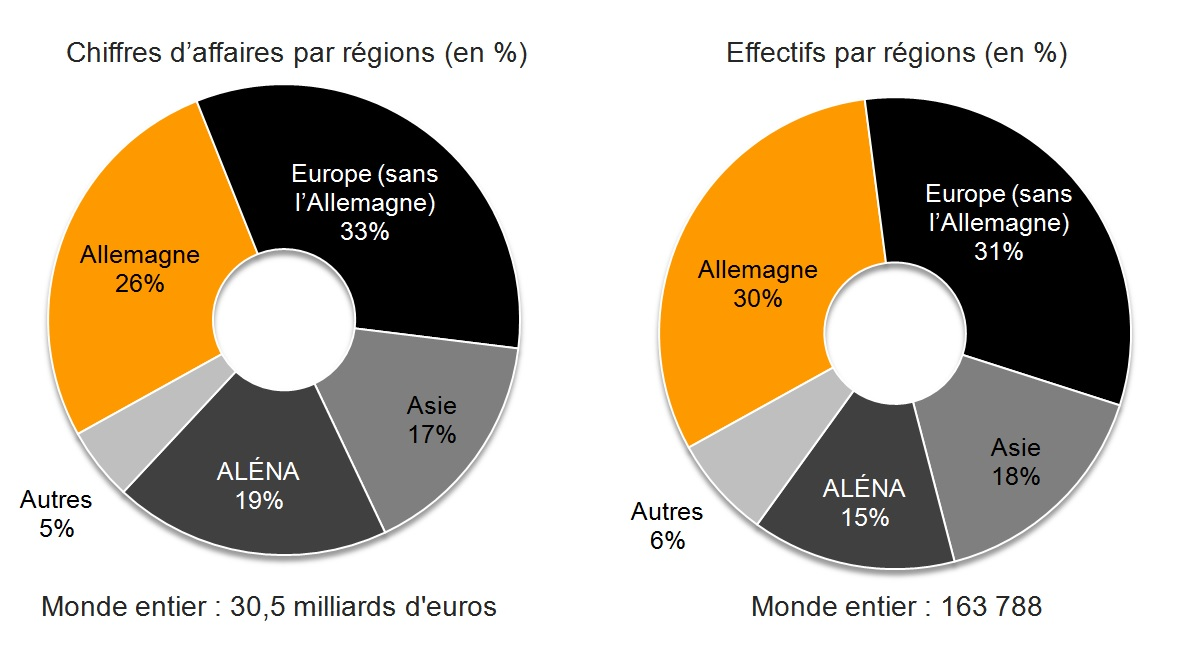
\includegraphics[width=12cm]{contents/images/caConti.jpg}
		 	\caption{Chiffre d'affaire et nombre d'employés}
		 	\label{fig:caConti}
		 \end{figure}

		 En 2011, l'entreprise comptait plus de $163000$ employés dans le monde\footnote{Cf figre \ref{fig:caConti}} répartis dans 269 sites et 46 pays différents\footnote{Cf figure \ref{fig:repartitionConti}}. Avec un chiffre d'affaire de 30.5 milliards d'euros au total, Continental est numéro un du marché de production de pneus en Allemagne et est également un important équipementier automobile.
		 \begin{figure}[H]
		 	\centering
		 	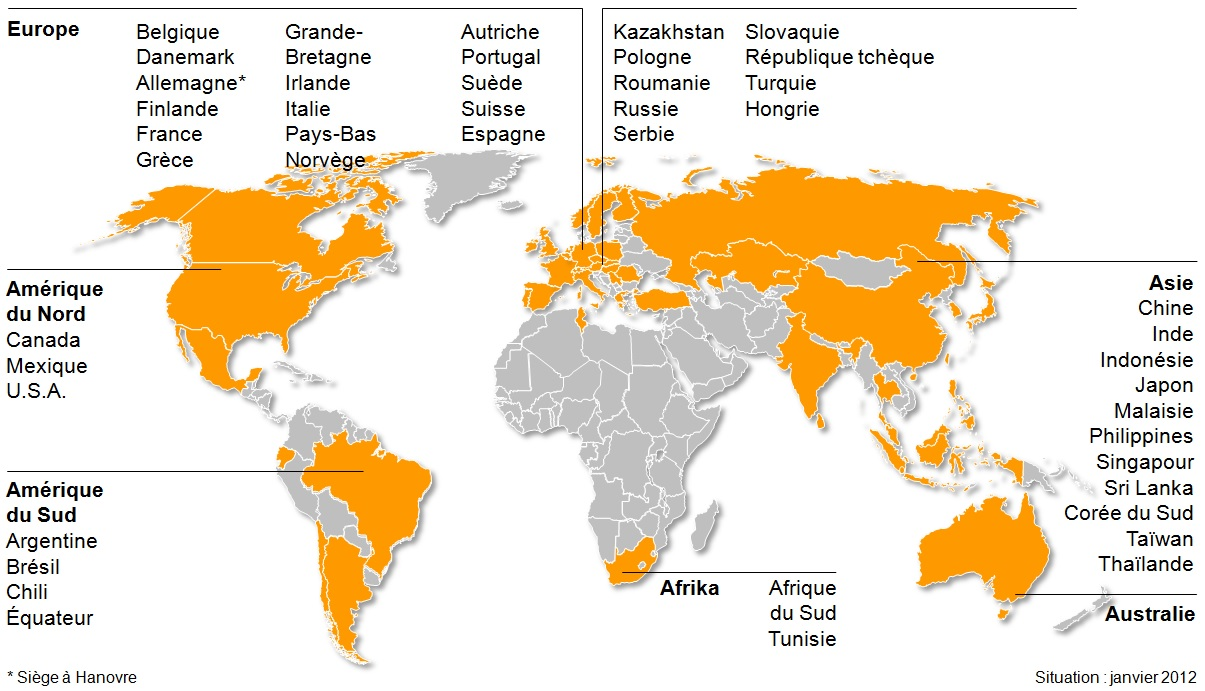
\includegraphics[width=13cm]{contents/images/repartitionConti.jpg}
		 	\caption{Répartition du groupe continental dans le monde}
		 	\label{fig:repartitionConti}
		 \end{figure}		 

		\subsection{Histoire de l'entreprise}
		Continental est fondée en 1871 comme société anonyme sous le nom de <<Continental-Caoutchouc-und Gutta-Percha Compagnie>> par neuf banquiers et industriels de Hanovre (Allemagne).

		Continental dépose l'emblème du cheval\footnote{Cf figure \ref{fig:logo}} comme marque de fabrique à l'Office impérial des brevets de Hanovre en octobre 1882. Il est aujourd'hui encore protégé en tant que marque distinctive.
		\begin{figure}[H]
			\centering
			
\includegraphics[width=2cm]{contents/images/logo.jpg}
			\caption{Logo de Continental}
			\label{fig:logo}
		\end{figure}

		Le fabricant de pneus allemand débute son expansion à l'international en tant que sous-traitant automobile international en 1979, expansion qu'il n'a cessé de poursuivre depuis.
		
Entre 1979 et 1985, Continental procède à plusieurs rachats qui permettent son essor en Europe, celui des activités pneumatiques européennes de l'américain Uniroyal Inc. et celui de l'autrichien Semperit.

En 1995 est créée la division << Automotive Systems >> pour intensifier les activités << systèmes >> avec l'industrie automobile.

La fin des années 1990 marque l'implantation de Continental en Amérique latine et en Europe de l'Est.

En 2001, pour renforcer sa position sur les marchés américain et asiatique, l'entreprise fait l'acquisition du spécialiste international de l'électronique Temic, qui dispose de sites de production en Amérique et en Asie. La même année, la compagnie reprend la majorité des parts de deux entreprises japonaises productrices de composants d'actionnement des freins et de freins à disques. 

En 2004, le plus grand spécialiste mondial de la technologie du caoutchouc et des plastiques naît de la fusion entre Phoenix AG et Conti'Tech.

Enfin en juillet 2007, Continental réalise sa plus grosse opération en rachetant le fournisseur automobile Siemens VDO Automotive. Ce rachat a permis à l'entreprise de multiplier son chiffre d'affaire par deux, passant ainsi de 13 milliards d'euros à plus de 30 milliards d'euros (chiffre de 2011).
		
		\subsection{Activités des différentes branches}
		\begin{figure}[H]
			\centering
			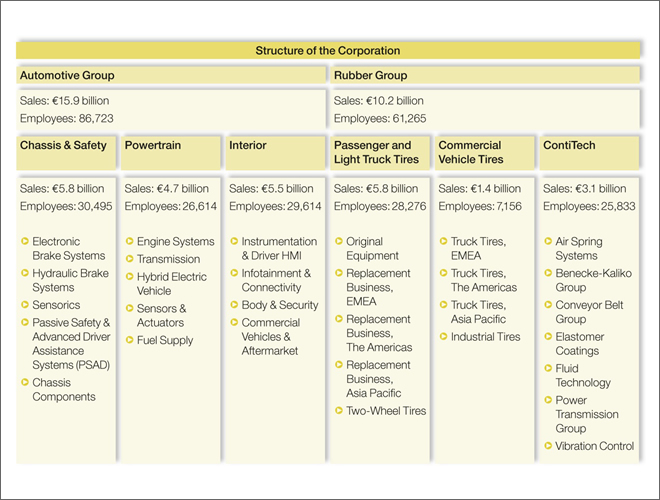
\includegraphics[width=18cm]{contents/images/structureConti.jpg}
			\caption{Structure de continental}
			\label{fig:structConti}
		\end{figure}

		Comme on peut le voir sur la figure \ref{fig:structConti}, Continental est composée de deux groupes et de six divisions. Ces dernières se chargent de développer et produire des équipements répondant aux besoins des clients. Pour cela elles sont composées de Business Units qui ont chacune une activité bien particulière dans leur domaine de compétence. 

Durant mon stage, je travaillais au sein de la division \textit{powertrain}. Elle s'occupe essentiellement du contrôle moteur, au niveau logiciel et materiel avec l'ECU\footnote{Electronic Control Unit} et de la mise au point des systèmes diesel et essence. Par exemple, la Business Unit <<Engine Systems>> est chargée de produire les équipements nécessaires au contrôle moteur tels que des calculateurs ou des 
injecteurs.

	\section{Le contexte de l'équipe Vérification \& Validation}
		\subsection{L'équipe}
		J'ai travaillé dans l'équipe en charge de la vérification et de la validation des logiciels.\footnote{Plus précisément dans le service P-ES-E-SYS-ETV-V.\newline P: Powertrain\newline ES-E-SYS: Engine Systems\newline ETV: Engineering Tool and Verification\newline V: Vérification.} dirigée par Stéphane \bsc{Bride}. Cette équipe est en charge du développement, de la configuration et de l'exécution de scripts de tests de régression automatique\footnote{Aussi appelés FaST : Functions and Software Testing} sur bancs HIL\footnote{Hardware in the Loop} avant la livraison des projets.
		
		\subsection{Le besoin} \label{besoinTests}
		Le calculateur du contrôle moteur d'une voiture est un dispositif très important et à haut risque, puisqu'une défaillance peut provoquer la mort de plusieurs personnes. Ainsi, le test est indispensable dans ce domaine, et doit être robuste. 

L'automatisation des tests est rendue nécessaire pour deux raisons. Tout d'abord, un logiciel ne peut comporter aucun bug, cependant les erreurs et bugs critiques liés à l'inattention peuvent être grandement réduits grâce à ce processus. De plus, au vue du très grand nombre de cas à tester pour un contrôle moteur, une opération manuelle serait impensable. 

C'est dans ce contexte que l'équipe Vérification et Validation intervient, elle doit fournir des outils aux développeurs afin de vérifier facilement et correctement leur travail, particulièrement pour des tests de régression, bien que l'outil que l'équipe est en train de développer soit à destination de tests d'intégration.

\setcounter{mtc}{3}
	\chapter{Organisation du travail}
\section{L'équipe de développement}
Au cours de mon stage, trois développeurs travaillaient sur le projet \textit{GreenT} : Alain \bsc{Fernandez}, chef d’équipe et membre de l’équipe Vérification et Validation, Olivier \bsc{Ramel}, sous-traitant de chez SII, et moi-même, stagiaire au sein de l’équipe Vérification et Validation.

En tant que chef d’équipe, Alain \bsc{Fernandez} organisait les réunions et supervisait notre travail tout en développant les tests managers\footnote{Cf \ref{testManager}}. Olivier \bsc{Ramel} se chargeait particulièrement de la partie serveur. Quant à moi je m’occupais de la partie parsing et génération\footnote{Cf \ref{generation}}.

À mon arrivée la conception du logiciel avait été commencée par mes deux collègues qui m’ont tous les deux formé afin que je puisse rapidement être opérationnel.

Ensemble nous avons convenu d’une réunion hebdomadaire tous les lundis matin afin de pouvoir faire un point sur nos avancements ou problèmes. Cela nous a permis d’avoir toujours une bonne vision du projet et de régler, ensemble, les problèmes au fur et à mesure. Pour autant, des réunions ponctuelles ont dû être organisées pour compléter ou revoir la conception en fonction des difficultés rencontrées durant la phase de développement.

\section{Documentation}
Une documentation, compte rendu des besoins du client et de tous nos choix de conceptions, a été mise en place au travers d’un document au format Word. Ainsi une
trace de toutes nos réunions et de notre conception est accessible sur un disque réseau. Elle permet à l'équipe de consulter les détails de ce qui avait été décidé plusieurs semaines auparavant.

\section{Outils de développement}
Afin de travailler de façon efficace, nous avons utilisés des outils aidant au développement.

\begin{wrapfigure}{r}{2cm}
	
\includegraphics[width=2cm]{contents/images/logoJava.png}
\end{wrapfigure}
La partie client de notre plateforme est développée en Java à sa version 6, Java nous permettant d'avoir un langage fortement typé, très puissant au niveau du paradigme Objet, connu de l'équipe, assez simple de déploiement et multiplateforme. 

Les postes de Continental possédant pour la plupart Java 6, aucune fonctionnalité ultérieur à cette version n'a été utilisé.\\~

\begin{wrapfigure}{l}{2.5cm}
	
\includegraphics[width=2.5cm]{contents/images/logoGit.png}
\end{wrapfigure}
Nous avons utilisé Git afin de faciliter le travail collaboratif d'une part, et de versionner le code du logiciel d'autres part. Git permet de fusionner les
modifications de plusieurs développeurs, tant que nous ne modifions pas le même fichier en même temps. Ainsi, la fusion de nos modifications était faite automatiquement. 

De plus, à chaque fois que nous effectuons une modification, nous faisons un << commit >>, dès lors un point de restauration se créé : il est possible de
récupérer n'importe quelle version de logiciel depuis son commencement. Nous y insérons un message clair expliquant ce que l'on à fait, cela permet aux autres développeurs de l'équipe de se tenir au courant de l'avancement.

\begin{wrapfigure}{r}{2.5cm}
	
\includegraphics[width=2.5cm]{contents/images/logoEclipse.png}
\end{wrapfigure}
Nous développions tous sous l'IDE\footnote{Integrated Development Tools} Eclipse Kepler, avec le plugin Git et le plugin PyDev. Le plugin Git permet d’avoir des outils aidant à la résolution d’éventuels conflits et le plugin PyDev permet de développer avec l’interpréteur et la coloration syntaxique Python. Je me suis rarement servi de ce dernier, mais il était indispensable pour développer la partie serveur de notre plateforme, qui fonctionne en Python. 

Notre plateforme fonctionne avec une architecture client-serveur, le client écrit en Java et le serveur utilise Python. Afin de faire communiquer les deux parties de notre application, nous avons utilisé Apache Thrift. Une bibliothèque ayant pour but les communications réseau inter-langage, dans le même principe que le protocole RMI\footnote{Remote Method Invocation}.

\begin{wrapfigure}{l}{2.5cm}
	
\includegraphics[width=2.5cm]{contents/images/logoEnterpriseArchitect.png}
\end{wrapfigure}
Nous avons travaillé avec la norme UML\footnote{Unified Modelling Language}~2 afin de concevoir la plateforme, en utilisant particulièrement des diagrammes de classes, mais aussi des diagrammes de cas d'utilisations ou d'activité. 

Pour dessiner ces diagrammes, et les noter dans la documentation, nous les pensions d'abord sur tableau blanc, mais ensuite nous avions besoin d'un outil puissant afin de les dessiner sur informatique. Pour cela nous avons utilisés Enterprise Architect, un logiciel propriétaire permettant de créer tous les diagrammes de la norme UML~2.\\~

\begin{wrapfigure}{r}{2.5cm}
	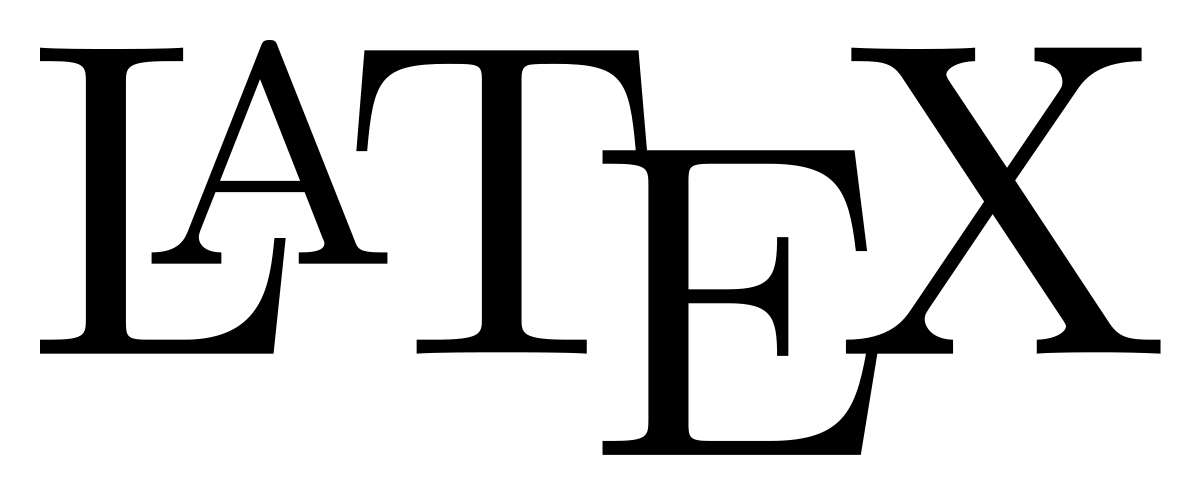
\includegraphics[width=2.5cm]{contents/images/logoLatex.png}
\end{wrapfigure}
Afin de rédiger ce rapport, et le diaporama de soutenance, j'ai utilisé \LaTeX{}, un langage et un système de composition de documents fonctionnant à l'aide de
macro-commandes. Son principal avantage est de privilégier le contenu à la mise en forme, celle-ci étant réalisée automatiquement par le système une fois un style définit. 
	
	\setcounter{mtc}{4}
	\chapter{Le problème} \label{chapPb}
\begin{wrapfigure}{r}{0.60\textwidth}
\vspace{-25px}
\hspace{-30px}
\begin{minipage}{0.67\textwidth}
\minitoc
\end{minipage}
\end{wrapfigure}
Depuis longtemps, l'entreprise avait un problème afin d'effectuer des tests d'intégrations, notamment pour les projets à destination de Ford. Les tests demandaient du temps et de l'argent à l'équipe en charge de ces tests. Ainsi, un an avant mon arrivée, une solution à été trouvée : le développement d'une nouvelle plateforme, \textit{GreenT}.

\vspace{-32px}
	\section{Les tests} \label{pbTests}
	Comme expliqué dans la section \ref{besoinTests}, le calculateur moteur est un système critique, il est donc indispensable de tester correctement celui-ci.

	\subsection{Le plugin}
	Dans le cadre de projets pour Ford, Continental ne développe pas l'intégralité du logiciel, en effet une partie est fournie par le client sous forme de << plugin >>. Le plugin est supposé correct, et ce n'est pas de notre ressort de le tester. Cependant, celui-ci va être interfacé avec les logiciels Continental : il est indispensable de vérifier que les deux parties fonctionnent ensemble lors de l'intégration.

	Pour cela, le client fourni un fichier appelé \texttt{Walkthrough}\footnote{Ce fichier est expliqué plus en détail section \ref{wt}} contenant la liste des variables du plugin avec toutes leur spécifications, ce fichier est au format \textit{Excel} : et il contient environ 900 variables différentes. Il est impensable de tester le fonctionnement d'autant de paramètres manuellement, ainsi l'équipe en charge de tester cette intégration effectue des tests de différence d'une version à l'autre : seules les variables ayant pu être impactées par une \textit{release} seront testées, il est supposé que les fonctionnement des variables restera inchangé.

	Trois problèmes se posent à cette méthode : 
	\begin{description}
		\item[La fiabilité des tests] Le test des seules différences ne permet pas nécessairement de détecter tous les problèmes (notamment avec des effets de bords…). De plus, une tâche répétitive peut entrainer des erreurs humaines.
		\item[Le temps de tests] Même en ne testant qu'une partie des variables, cela prend un temps considérable, il faut compter environ une semaine.
		\item[La disponibilité des bancs de tests]	Les tests s'effectuent sur des bancs de tests\footnote{Une photo d'un banc est disponible figure \ref{fig:photoHil}}, ces équipements permettent de simuler un environnement voiture autour du contrôleur moteur comme l'utilisation de la clé de démarrage, la tension de la batterie, la vitesse de rotation du moteur, ... Comme ces bancs de tests sont peu nombreux dans l'entreprise, en raison de leur coût et qu'il est nécessaire de réserver les bancs pendant une semaine afin d'effectuer les tests cette méthode peut bloquer d'autres personnes en ayant besoin.
	\end{description}
	\begin{figure}[H]
		\centering
		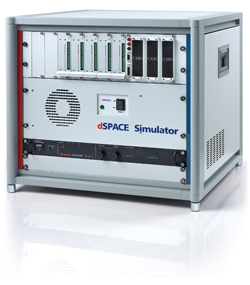
\includegraphics[width=7cm]{contents/images/hil.jpg}
		\caption{Exemple de banc de tests -- HIL DSpace}
		\label{fig:photoHil}
	\end{figure}

	\subsection{La plateforme TA3}
	Actuellement, les équipes de tests disposent d'une plateforme appelée TA3. Celle-ci est une bibliothèque de classes écrites en Python. Jusqu'à présent, pour chaque objectif de test, il fallait écrire un script python utilisant la TA3. Ces scripts pilotent le banc Hil et le l'outil de debug afin d'envoyer des stimulis à l'Unité de contrôle moteur(Noté ECU pour \textit{Electronic Control Unit}) et de vérifier que les réactions de celui-ci sont conforme aux spécifications de test.
	\begin{figure}[H]		
		\centering
		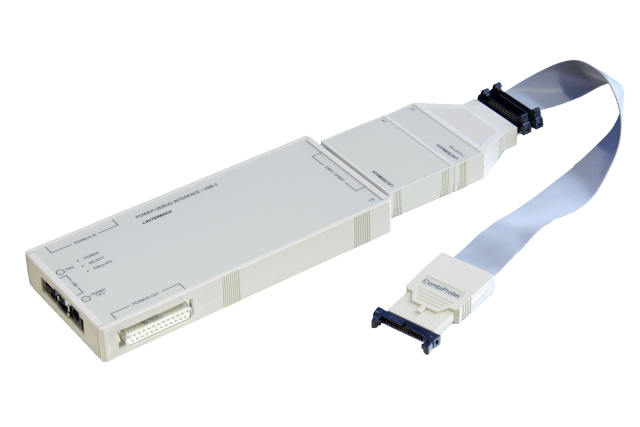
\includegraphics[width=7cm]{contents/images/trace32.png}
		\caption{Exemple de Debugger -- Trace32}
		\label{fig:photoHil}
	\end{figure}

	Cependant, cette plateforme pose un certain nombre de problèmes qui rend son utilisation difficile. D'une part, elle renvoie un trop grand pourcentage de faux-positifs, faisant perdre un temps considérable. D'autres part, elle ne prend pas en compte certains besoins apparu récemments Comme par exemple un système permettant de flasher automatiquement les ECU, ou la possibilité de vérifier la fréquence de mise-à-jour de la production de variables.
\\~

	Afin d'améliorer cette situation, l'équipe Vérification et Validation a décidé de développer une nouvelle plateforme.

	\section{La solution : \textit{GreenT}}
	Afin de résoudre les problèmes présentés dans la section \ref{pbTests}, une solution a été pensée avant mon arrivée en étudiant les besoins de l'équipe en charge des tests du plugin : le développement d'une plateforme de tests, appelé \textit{GreenT}.

	\subsection{Génération de tests automatiques}
	\subsubsection{Les tests d'intégration du plugin Ford}
	À court terme, cette solution devrait permettre de tester le plugin pour les projets Ford facilement et de façon efficace. Pour cela, les testeurs Continental vont ajouter des colonnes dans le document \texttt{walkthrough}, afin de spécifier la manière de tester les variables. La plateforme, sera capable d'analyser le document \texttt{walkthrough}, et de générer les tests automatiques. Le testeur n'aura plus qu'à lancer l'exécutable le soir, il reviendra le lendemain, tous les tests auront été exécutés avec un rapport détaillé pour chaque test.\\

	Ces tests s'effectueront sur des variables enregistrées lors de stimulation du contrôleur, afin de vérifier que celui-ci réagit de façon approprié.

	Cette plateforme permettra donc de tester facilement la dizaine de projets Ford, et une fois le test d'une variable spécifiée, il n'est plus nécessaire de le réécrire. À chaque nouvelle \textit{release} il suffira de relancer les tests : l'équipe n'aura à faire le travail qu'une fois, ensuite la réutilisation sera possible, les projets seront testés plus rapidement, plus efficacement, et plus souvent.

	\subsubsection{Les autres projets}
	À moyen terme, cette plateforme pourrait être utilisée pour les projets d'autres clients tel que Renault, afin d'effectuer là aussi des tests d'intégration, il est donc nécessaire de concevoir une plateforme qui puisse évoluer facilement, et avoir un fichier de spécifications en entrée qui soit légèrement différent d'un client à l'autre.

	En effet, les autres clients peuvent aussi fournir une partie du logiciel, avec un document de spécification des variables, celui-ci ne serait pas totalement identique, mais l'approche des tests s'en approchera.

	Il est également envisageable que la plateforme soit utilisée pour des tests d'intégration en interne, indépendamment des spécifications fournies par le client.

	\subsection{L'utilisation de \textit{GreenT} comme une bibliothèque}
		Une autre approche de notre plateforme, serait de s'en servir pour écrire facilemet des tests en Java, de façon plus efficace et plus robuste qu'avec la TA3 : notre plateforme doit donc également fonctionner comme une bibliothèque sans utilisation de générateur ou de parser, pour que le testeur puisse effectuer un test rapide. 

		Celui-ci apprendra à se servir de la plateforme, écrira en règle générale des tests assez courts et moins complexes que ceux que nous générerons, ceux-ci doivent être faciles à écrire.

	\subsection{L'exécution des tests}
	À long terme, l'objectif serait de pouvoir effectuer de l'intégration continue. 

	Il faut savoir que l'exécution de ces tests pourrait durer une quinzaine d'heures, en espérant qu'elle tienne sur une nuit. Cependant, il va arriver que les tests débordent et que lorsque le testeur revient, les tests ne soient pas terminés : le banc va être occupé alors que d'autres personnes en ont besoin, et le testeur n'a toujours pas les verdicts.

	 Nous souhaitons concevoir un système permettant l'exécution des tests sur des bancs en parallèle : on pourrait ainsi diviser le temps d'exécution par 2 ou 3, les tests tiendront sur une nuit et l'objectif principal serait tenu.

	 Mais le plus intéressant, serait d'utiliser le décalage horaire à notre avantage : lancer l'exécution des tests sur des bancs non utilisés dans d'autres pays, ainsi à toute heure de la journée il serait possible de lancer les tests. En effet, Continental étant présent dans la plupart des continents, il fait toujours nuit sur un site sur la planète. Après chaque étape d'intégration, on pourrait relancer les tests afin de vérifier qu'aucun bug n'a été introduit : le problème de la disponibilité des bancs serait alors résolu, et nous atteindrons une excellente sécurité.


	\setcounter{mtc}{5}
		\chapter{Développement de \textit{GreenT}}
		\section{Fonctionnement général}
			\subsection{Schéma de fonctionnement}
			\subsection{Le fichier Walkthrough}
			\subsection{Le test manager}
			\subsection{Découpage en Bundle}

		\section{Le parser}
			\subsection{La grammaire : utilisation de Antlr}
			\subsection{La visite de l'arbre d'expression}
			\subsection{La gestion des exceptions}
			% antlr
		\section{Le générateur}
			\subsection{Le moteur de template : freemaker}
			\subsection{Génération des tests}
			% freemaker

	\setcounter{mtc}{6}
	\chapter{Bilans}
	\lipsum[3]
	\section{Bilan pour Continental}
	\lipsum
	\section{Bilan personnel}
	\lipsum

	
	\appendix
	\chapter{Glossaire}
% HIL
% Trace32
% UML
% Logiciel de versionnement
% ECU
% JSON
% Thrift
% Grammaire
% Antlr
% Parser


		\chapter{Templates}\label{annexeTemplate}
	\section{Template des stimulations}
	\lstinputlisting[language=Java, caption=Template des stimulations]{contents/codes/ClassStimTemplate.ftl}
	\newpage
	\section{Template d'un \texttt{GreenTTest}}
	\lstinputlisting[language=Java, caption=Template d'un GreenTTest]{contents/codes/ClassGreenTTestGenerator.ftl}

		\chapter{Exemples de fichiers générés}\label{annexeGeneration}
	\section{Exemple de StimScenario}
	\lstinputlisting[language=Java, caption=Exemple de StimScenario]{contents/codes/StimScenario_Stub_1.java}
	\newpage
	\section{Exemple de \texttt{GreenTTest}}
	\lstinputlisting[language=Java, caption=Exemple de GreenTTest]{contents/codes/GreenTTest_AIRT_Air_uRawTCACDsB2.java}

	\lstlistoflistings
	\listoffigures

\end{document}
